\documentclass[english,man]{apa6}

\usepackage{amssymb,amsmath}
\usepackage{ifxetex,ifluatex}
\usepackage{fixltx2e} % provides \textsubscript
\ifnum 0\ifxetex 1\fi\ifluatex 1\fi=0 % if pdftex
  \usepackage[T1]{fontenc}
  \usepackage[utf8]{inputenc}
\else % if luatex or xelatex
  \ifxetex
    \usepackage{mathspec}
    \usepackage{xltxtra,xunicode}
  \else
    \usepackage{fontspec}
  \fi
  \defaultfontfeatures{Mapping=tex-text,Scale=MatchLowercase}
  \newcommand{\euro}{€}
\fi
% use upquote if available, for straight quotes in verbatim environments
\IfFileExists{upquote.sty}{\usepackage{upquote}}{}
% use microtype if available
\IfFileExists{microtype.sty}{\usepackage{microtype}}{}

% Table formatting
\usepackage{longtable, booktabs}
\usepackage{lscape}
% \usepackage[counterclockwise]{rotating}   % Landscape page setup for large tables
\usepackage{multirow}		% Table styling
\usepackage{tabularx}		% Control Column width
\usepackage[flushleft]{threeparttable}	% Allows for three part tables with a specified notes section
\usepackage{threeparttablex}            % Lets threeparttable work with longtable

% Create new environments so endfloat can handle them
% \newenvironment{ltable}
%   {\begin{landscape}\begin{center}\begin{threeparttable}}
%   {\end{threeparttable}\end{center}\end{landscape}}

\newenvironment{lltable}
  {\begin{landscape}\begin{center}\begin{ThreePartTable}}
  {\end{ThreePartTable}\end{center}\end{landscape}}

  \usepackage{ifthen} % Only add declarations when endfloat package is loaded
  \ifthenelse{\equal{\string man}{\string man}}{%
   \DeclareDelayedFloatFlavor{ThreePartTable}{table} % Make endfloat play with longtable
   % \DeclareDelayedFloatFlavor{ltable}{table} % Make endfloat play with lscape
   \DeclareDelayedFloatFlavor{lltable}{table} % Make endfloat play with lscape & longtable
  }{}%



% The following enables adjusting longtable caption width to table width
% Solution found at http://golatex.de/longtable-mit-caption-so-breit-wie-die-tabelle-t15767.html
\makeatletter
\newcommand\LastLTentrywidth{1em}
\newlength\longtablewidth
\setlength{\longtablewidth}{1in}
\newcommand\getlongtablewidth{%
 \begingroup
  \ifcsname LT@\roman{LT@tables}\endcsname
  \global\longtablewidth=0pt
  \renewcommand\LT@entry[2]{\global\advance\longtablewidth by ##2\relax\gdef\LastLTentrywidth{##2}}%
  \@nameuse{LT@\roman{LT@tables}}%
  \fi
\endgroup}


  \usepackage{graphicx}
  \makeatletter
  \def\maxwidth{\ifdim\Gin@nat@width>\linewidth\linewidth\else\Gin@nat@width\fi}
  \def\maxheight{\ifdim\Gin@nat@height>\textheight\textheight\else\Gin@nat@height\fi}
  \makeatother
  % Scale images if necessary, so that they will not overflow the page
  % margins by default, and it is still possible to overwrite the defaults
  % using explicit options in \includegraphics[width, height, ...]{}
  \setkeys{Gin}{width=\maxwidth,height=\maxheight,keepaspectratio}
\ifxetex
  \usepackage[setpagesize=false, % page size defined by xetex
              unicode=false, % unicode breaks when used with xetex
              xetex]{hyperref}
\else
  \usepackage[unicode=true]{hyperref}
\fi
\hypersetup{breaklinks=true,
            pdfauthor={},
            pdftitle={LAB: Linguistic Annotated Bibliography -- A searchable portal for normed database information},
            colorlinks=true,
            citecolor=blue,
            urlcolor=blue,
            linkcolor=black,
            pdfborder={0 0 0}}
\urlstyle{same}  % don't use monospace font for urls

\setlength{\parindent}{0pt}
%\setlength{\parskip}{0pt plus 0pt minus 0pt}

\setlength{\emergencystretch}{3em}  % prevent overfull lines

\ifxetex
  \usepackage{polyglossia}
  \setmainlanguage{}
\else
  \usepackage[english]{babel}
\fi

% Manuscript styling
\captionsetup{font=singlespacing,justification=justified}
\usepackage{csquotes}
\usepackage{upgreek}

 % Line numbering
  \usepackage{lineno}
  \linenumbers


\usepackage{tikz} % Variable definition to generate author note

% fix for \tightlist problem in pandoc 1.14
\providecommand{\tightlist}{%
  \setlength{\itemsep}{0pt}\setlength{\parskip}{0pt}}

% Essential manuscript parts
  \title{LAB: Linguistic Annotated Bibliography -- A searchable portal for normed
database information}

  \shorttitle{Linguistic Bibliography}


  \author{Erin M. Buchanan\textsuperscript{1}, Kathrene D. Valentine\textsuperscript{2}, \& Nicholas P. Maxwell\textsuperscript{1}}

  % \def\affdep{{"", "", ""}}%
  % \def\affcity{{"", "", ""}}%

  \affiliation{
    \vspace{0.5cm}
          \textsuperscript{1} Missouri State University\\
          \textsuperscript{2} University of Missouri  }

  \authornote{
    Erin M. Buchanan is an Associate Professor of Quantitative Psychology at
    Missouri State University. K. D. Valentine is a Ph.D.~candidate at the
    University of Missouri. Nicholas P. Maxwell is a Masters' candidate at
    Missouri State University. We thank Michael T. Carr, Farren E.
    Bankovich, Samantha D. Saxton, and Emmanuel Segui for their help with
    the original data processing, and William Padfield, Abigial Van Nuland,
    and Abbie Wikowsky for their help with the application develop for the
    website.
    
    Correspondence concerning this article should be addressed to Erin M.
    Buchanan, 901 S. National Ave, Springfield, MO 65897. E-mail:
    \href{mailto:erinbuchanan@missouristate.edu}{\nolinkurl{erinbuchanan@missouristate.edu}}
  }


  \abstract{In the era of big data, psycholinguistic research is flourishing with
numerous publications that advance our knowledge of concept
characteristics and ways to study them. This article presents the
Linguistic Annotated Bibliography (LAB) as a searchable web portal to
quickly and easily access reliable database norms, related programs, and
variable calculations. These publications (\emph{N} = 706) were coded by
language, number of stimuli, stimuli type (i.e., words, pictures,
symbols), keywords (i.e., frequency, semantics, valence), and other
useful information. This tool not only allows researchers to search for
the specific type of stimuli needed for experiments, but also permits
the exploration of publication trends across 100 years of research.
Details about the portal creation and use are outlined, as well as
various analyses of change in publication rates and keywords. In
general, advances in computation power have allowed for the increase in
dataset size in the recent decades, in addition to an increase in the
number of linguistic variables provided in each publication.}
  \keywords{database, stimuli, online portal, megastudy, trends \\

    
  }





\usepackage{amsthm}
\newtheorem{theorem}{Theorem}
\newtheorem{lemma}{Lemma}
\theoremstyle{definition}
\newtheorem{definition}{Definition}
\newtheorem{corollary}{Corollary}
\newtheorem{proposition}{Proposition}
\theoremstyle{definition}
\newtheorem{example}{Example}
\theoremstyle{definition}
\newtheorem{exercise}{Exercise}
\theoremstyle{remark}
\newtheorem*{remark}{Remark}
\newtheorem*{solution}{Solution}
\begin{document}

\maketitle

\setcounter{secnumdepth}{0}



The advance of computational ability and the Internet have propelled
research into an era of \enquote{big data} that has interesting
implications for the field of psycholinguistics, as well as other
experimental areas that use normed stimuli for their research.
Traditionally, stimuli used for experimental psycholinguistics research
were first normed through small in-house pilot studies, which were then
used in many subsequent projects. While economic, this selection
procedure's results could be potentially misleading as a factor of the
stimuli, rather than experimental manipulation. Small individual lab
norming projects may be tied to a lack of funding, time, computational
power, or even interest in studying phenomena at the stimuli level. Now,
we have the capability to collect, analyze, and publish large datasets
for research into memory models (Cree, McRae, \& McNorgan, 1999; Moss,
Tyler, \& Devlin, 2002; Rogers \& McClelland, 2004; Vigliocco, Vinson,
Lewis, \& Garrett, 2004), aphasias (Vinson, Vigliocco, Cappa, \& Siri,
2003), probability and linguistics (Cree \& McRae, 2003; McRae, De Sa,
\& Seidenberg, 1997; Pexman, Holyk, \& Monfils, 2003), valence (Dodds,
Harris, Kloumann, Bliss, \& Danforth, 2011; Vo et al., 2009; Warriner,
Kuperman, \& Brysbaert, 2013), and reading speeds and priming (Balota et
al., 2007; Cohen-Shikora, Balota, Kapuria, \& Yap, 2013; Hutchison et
al., 2013; Keuleers, Lacey, Rastle, \& Brysbaert, 2012) to name a small
subset of research avenues.

Big data has manifested in psycholinguistics over the last decade in the
form of grant funded megastudies to collect and analyze large text
corpora (i.e., the SUBTLEX projects) or to examine numerous word
properties in one study (i.e., the Lexicon projects). The SUBTLEX
projects were designed to analyze frequency counts for concepts across
extremely large corpora sizes using subtitles as a substitute for
natural speech. The investigation of these measures was first spurred by
the realization that word frequency is an important predictor of naming
and lexical decision times (Balota, Cortese, Sergent-Marshall, Spieler,
\& Yap, 2004; Rayner \& Duffy, 1986). While previous measures of
frequency (i.e., Baayen, Piepenbrock, Gulikers, \& Linguistic Data
Consortium, n.d.; Burgess \& Livesay, 1998; Kucera \& Francis, 1967)
were based on large one million+ word corpora, they were poor predictors
of response latencies (Balota et al., 2004; Brysbaert \& New, 2009;
Zevin \& Seidenberg, 2002). Further, it appears from Brysbaert and New
(2009)'s investigation into corpora size and type, that not only should
the corpora be large (\textgreater{}sixteen million), but the underlying
source of the text data matters (Internet versus subtitles), as well as
the contextual diversity of the data (i.e., number of occurrences across
sources; Adelman, Brown, \& Quesada, 2006). Not only has Brysbaert and
New (2009)'s work been included in newer lexical studies (Hutchison et
al., 2013; Yap, Tan, Pexman, \& Hargreaves, 2011), but SUBTLEX projects
have been published in Dutch (Keuleers, Brysbaert, \& New, 2010), Greek
(Dimitropoulou, Duñabeitia, Avilés, Corral, \& Carreiras, 2010), Spanish
(Cuetos, Glez-Nosti, Barbon, \& Brysbaert, 2011), Chinese (Cai \&
Brysbaert, 2010), French (New, Brysbaert, Veronis, \& Pallier, 2007),
British English (Heuven, Mandera, Keuleers, \& Brysbaert, 2014), and
German (Brysbaert et al., 2011).

The Lexicon projects involved creating large databases of validated
mono- and multisyllabic words to assist in the creation of controlled
experimental stimuli sets for future experiments. These databases
contain lexical decision and naming response latencies, as well as
typical word confound variables such as orthographic neighborhood,
phonological, and morphological characteristics. While the English
Lexicon Project (Balota et al., 2007) is the most cited of the lexicons,
other languages include Chinese (Sze, Rickard Liow, \& Yap, 2014), Malay
(Yap, Rickard Liow, Jalil, \& Faizal, 2010), Dutch (Keuleers et al.,
2010), and British English (Keuleers et al., 2012). Another twenty or so
similar lexical database publications can be found in the literature
covering French (Lété \& Sprenger-Charolles, 2004), Italian (Barca,
Burani, \& Arduino, 2002), Arabic (Boudelaa \& Marslen-Wilson, 2010),
and Portuguese (Soares et al., 2014).

The availability of big data has augmented the psycholinguistic
literature, but these projects are certainly time consuming due to the
amount of participant data required to achieve reliable and stable
norms. A solution to large data collection lies in several avenues of
easily obtainable data. First, Amazon's Mechanical Turk, an online crowd
sourcing avenue that allows researchers to pay users to complete
questionnaires, has shown to be a reliable, diverse participant pool
made available at very low cost (Buhrmester et al., 2011; Mason \& Suri,
2012). Researchers can pre-screen for specific populations, as well as
post-screen surveys for incomplete or inappropriate responses (Buchanan
\& Scofield, 2018), thus saving time and money with the elimination of
poor data. Because of the popularity of Mechanical Turk, large amounts
of data can be collected in shorter time periods than traditional
experiments. Mechanical Turk has been used to collect data for semantic
word pair norms (Buchanan, Holmes, Teasley, \& Hutchison, 2013), age of
acquisition ratings (Kuperman, Stadthagen-Gonzalez, \& Brysbaert, 2012),
concreteness ratings (Brysbaert, Warriner, \& Kuperman, 2014), past
tense information (Cohen-Shikora et al., 2013), and valence and arousal
ratings (Dodds et al., 2011; Jasmin \& Casasanto, 2012; Warriner et al.,
2013). Additionally, in a similar vein to the SUBTLEX projects,
linguistic data has been mined from open source data, such as the New
York Times, music lyrics, and Twitter (Dodds et al., 2011; Kloumann,
Danforth, Harris, Bliss, \& Dodds, 2012). Finally, De Deyne, Navarro,
and Storms (2013) have seen success in simply setting up a special
website (www.smallworldofwords.com) to gamify the collection of word
pair association norms.

The evolution of big data provides exciting opportunities for
exploration into psycholinguistics, and this article features the trends
in publications of normed datasets across the literature, allowing for a
large-scale picture of the developments of trends in psychological
stimuli. Historically, these norms have been published in journals
connected to the Psychonomic Society, such as Behavior Research Methods,
Psychonomic Monograph Supplements, and Perception and Psychophysics. The
society once hosted an electronic database that contained the links to
these norms, as well as a search tool to find information about
previously published works (Vaughan, 2004). The sale of the society
journals to Springer publications has improved journal visibility and
user-friendly access, but also has left a need for an indexed list of
database publications that span multiple keywords and journal websites.
Therefore, the purpose of this article is twofold: 1) to present a
searchable, cataloged database of normed stimuli and related materials
for a wide range of experimental research, and 2) to examine trends in
the publications of these articles to assess the big data movement
within cogntive psychology.

\section{Website}\label{website}

This manuscript was written with \emph{R} markdown and Aust and Barth
(2017) and can be found at \url{https://osf.io/9bcws/}. Readers can find
the website by going to \url{http://www.wordnorms.com}, and the source
files for the website can be found at
\url{https://github.com/doomlab/wordnorms}. From the webpage, the top
navigation bar includes a link to direct the reader to the LAB page. On
the LAB page, we have included a purpose statement and several summary
options. First, the variable tables include summary descriptions about
the stimuli and keyword (tags) variables in this study. The links
redirect to Shiny applications. Shiny is an open source graphical user
interface \emph{R} package that allows researchers to build interactive
web applications (Chang, Cheng, Allaire, Xie, \& McPherson, 2017). These
apps connect to the LAB database and display the current \emph{N},
minimum, maximum, mean and standard deviation for each variable, when
appropriate. The advantage to using Shiny apps is dynamic updating of
the database, so as new information is added, the app will display the
most current statistics. Viewers can suggest articles that should be
included in the dataset by using the email link included on the website.
The entire dataset can be viewed and filtered based on keyword,
language, and stimuli type. This search app allows for multiple filter
options, so a person may drill down into very specific search criteria.
Underneath the search functions, yearly trend visualization and
descriptive statistics may be found including frequency tables of
stimuli and keywords. Finally, the complete database in csv format can
be downloaded. Specific features will be outlined below in relation to
the database creation.

\section{Database Methods}\label{database-methods}

\subsection{Materials}\label{materials}

Bradshaw (1984) and Proctor and Kim-Phuong (1999)'s lists of database
information were used as starting points for collection of research
articles. We searched \emph{Academic Search Premier, PsycInfo, and ERIC}
through the EBSCO host system, as well as \emph{Google Scholar and PLoS
One} to find other relevant articles using the following keywords:
\emph{corpus, linguistic database, linguistic norms, norms, and
database}. Additionally, since many of the original articles were hosted
by the Psychonomic Society, the Springer website was searched with these
terms that covered the newer editions of \emph{Behavior Research
Methods} and \emph{Memory \& Cognition}. We then filtered for articles
that met the following criteria: 1) contained database information as
supplemental material, 2) demonstrated programs related to building
research stimuli using normed databases, or 3) generated new
calculations of lexical variables. Research articles that used normed
databases in experimental design or tested those variables
validity/reliability were excluded if they did not include new database
information. Additional articles were found while coding initial
publications by searching citations for stimuli selection. For example,
the Snodgrass and Vanderwart (1980) norms were cited in many newer
articles on line drawings, and therefore this article was subsequently
entered into the database. At the time of writing, 706 articles, books,
websites, and technical reports were included in the following analyses.

\subsection{Coding Procedure}\label{coding-procedure}

The tables with summaries from Bradshaw (1984) and Proctor and
Kim-Phuong (1999) were consulting for a starting point for data coding.
Next, the first round of articles found (approximately 100) were
analyzed to determine information that would be pertinent to a user who
wished to search for normed stimuli. Based on these reviews and lab
discussions, we coded the following information from each article: 1)
journal information, 2) stimuli types, 3) stimuli language, 4) programs
or corpus name, 5) keywords, which we refer to as tags, 6) special
populations, and 7) other notes that did not fit into those categories.
Each piece of information is detailed below. In some instances, codes
were not used as frequently as expected based on these initial
discussions, but were included to allow more specificity in searching,
as well as the flexibility to include those options for articles
subsequently added to the database.

\subsubsection{Journal Information}\label{journal-information}

Each article was coded with the citation information, and a complete
list of citations can be found on the website portal by clicking on view
and search data. All author last names are listed, along with
publication year, article title, journal title, volume, page numbers,
and digital object identifier (DOI) when available. This information is
listed in citation format in the Shiny app and separated into columns in
the downloadable data for easier sorting and searching. For newer
articles that have been published online first without volume or page
numbers, X and XX-XX are used as placeholders until official
publication. Although APA style dictates et al. for references after the
second author or immediately for large author publications, all names
were included each time they were referenced (see below). The inclusion
of these names allows a user to search for specific researchers, as well
as separates different publications by the same first author. A complete
list of publication sources, number of times cited, and percentages can
be found online by using the frequency statistics link.

\subsubsection{Stimuli Types}\label{stimuli-types}

While this publication was originally intended for traditional
linguistic database norms, other types of experimental stimuli used in
concept studies were apparent after background review. Therefore,
stimuli were coded based on the dominant description from the article
(i.e., although heteronyms are words and word pairs, they were coded
specifically as heteronyms). The number of stimuli presented in the
appendix or database was coded with the stimuli, unless the article
covered specific programs, search or experimental creation tools, which
is the majority of the \enquote{other} stimuli category. Because many
articles included two types of stimuli, or references to different
articles where stimuli were selected from, two options for stimuli were
included. Therefore, the total values for number of stimuli do not add
up to the number of articles in the database because of multiple
instances in articles or no stimuli for program descriptions. Table
\ref{tab:stim-table} includes a stimuli list, the number of times that
each stimuli was used, percentage of the total stimuli codes, the mean
and standard deviation of the number of those stimuli, minimum, maximum,
and a brief variable description. Researchers often cited specific
previous works where stimuli were selected from, and these references
were included, which can be found in the downloaded data. Table
\ref{tab:stim-table} is included dynamically online under view the
variable table and view the frequency table.

\begin{table}[tbp]
\begin{center}
\begin{threeparttable}
\caption{\label{tab:stim-table}Stimuli Definitions and Descriptive Statistics}
\begin{tabular}{llcccccc}
\toprule
Stimuli & \multicolumn{1}{c}{Description} & \multicolumn{1}{c}{N} & \multicolumn{1}{c}{Minimum} & \multicolumn{1}{c}{Maximum} & \multicolumn{1}{c}{M} & \multicolumn{1}{c}{SD} & \multicolumn{1}{c}{Percent}\\
\midrule
Anagrams & Words whose letters can be rearranged into other real words. & 6.00 & \ \  80.00 & 3.8e+02 & \ \ \ \ 229.00 & 2.1e+02 & 0.8\\
Categories & Lists of words that are associated with particular category names, such as animals & 31.00 & \ \ \ \ 4.00 & 2.4e+02 & \ \ \ \  43.41 & 4.7e+01 & 4.0\\
Characters & Characters are non-Roman letters, usually Japanese or Chinese logographs. & 21.00 & \ \  48.00 & 4.7e+07 & 2480334.00 & 1.1e+07 & 2.7\\
Cloze/Sentences & Sentence norms are complete or partial sentences in structure. Cloze norms are sentences with a missing word, and probabilities of different words to complete that blank are provided.. & 35.00 & \ \ \ \ 5.00 & 2.0e+03 & \ \ \ \ 353.66 & 3.8e+02 & 4.5\\
Color drawings & Line drawings or similar non-picture images that are colored. & 9.00 & \ \ 200.00 & 7.4e+02 & \ \ \ \ 384.00 & 2.1e+02 & 1.2\\
Homo/Heterographs & Homographs are two words with the same spelling, often with different pronunciations, and different meanings (bow), while heterographs have different spellings and meanings (to, two). & 10.00 & \ \  20.00 & 5.7e+02 & \ \ \ \ 161.44 & 1.8e+02 & 1.3\\
Homo/Heteronyms & Homonyms have the same spelling and pronunciation, but have different meanings (bank), while heteronyms have the same spelling with different pronunciations and meanings (desert). & 5.00 & \ \ 114.00 & 5.8e+02 & \ \ \ \ 343.75 & 2.5e+02 & 0.6\\
Homo/Heterophones & Homophones have the same pronunciation but different meanings (rose), while heterophones are often considered heteronyms with the same spelling but different pronunciations and meanings. & 3.00 & \ \  40.00 & 2.1e+02 & \ \ \ \ 148.00 & 9.4e+01 & 0.4\\
Letters & Alphabetic written elements. & 56.00 & \ \ \ \ 9.00 & 8.8e+03 & \ \ \ \ 679.08 & 1.6e+03 & 7.2\\
Line drawings & A non-picture image that is not colored. & 42.00 & \ \  22.00 & 5.2e+02 & \ \ \ \ 243.83 & 1.3e+02 & 5.4\\
Names & Words that are traditionally considered first or last names, such as Bob and Smith. & 7.00 & \ \ 126.00 & 1.0e+04 & \ \  2644.17 & 4.1e+03 & 0.9\\
Other & This category was used for stimuli that did not fit into others, programs or experimental stimuli creation tools, and each is described in the online table with that particular row in stimuli notes. & 50.00 & \ \ \ \ 1.00 & 3.1e+03 & \ \ \ \ 720.89 & 9.2e+02 & 6.5\\
Phonemes & A basic unit of sound in a language wherein changes bring changes to a word's meaning. & 4.00 & 10000.00 & 1.0e+04 & \ \ 10000.00 & \ \ \ \  NA & 0.5\\
Pictures & Photographs or other complex images. & 62.00 & \ \ \ \ 2.00 & 2.9e+03 & \ \ \ \ 417.45 & 4.7e+02 & 8.0\\
Pseudowords & Non-real words that are often created by changing one letter of a real word to create a linguistically valid consonant-vowel combination (wug). & 12.00 & \ \  30.00 & 4.0e+04 & \ \ 12887.78 & 1.6e+04 & 1.5\\
Sounds & Clips of noises, speech, or songs. & 8.00 & \ \  22.00 & 1.7e+02 & \ \ \ \ 117.00 & 4.9e+01 & 1.0\\
Syllables & A unit of pronunciation with at least one vowel, dipthong, or consonant. & 9.00 & \ \  33.00 & 1.4e+05 & \ \ 18129.00 & 4.9e+04 & 1.2\\
Symbols/Icons & Non-word characters. & 5.00 & \ \  68.00 & 6.0e+02 & \ \ \ \ 308.75 & 2.2e+02 & 0.6\\
Word Pairs & Words that were specifically paired for study in the article, such as studies on priming or word association. & 28.00 & \ \  40.00 & 7.2e+04 & \ \  8076.83 & 2.1e+04 & 3.6\\
Words & A distinct meaningful element of speech or writing. & 372.00 & \ \  10.00 & 5.9e+08 & 6964032.05 & 4.6e+07 & 48.0\\
\bottomrule
\end{tabular}
\end{threeparttable}
\end{center}
\end{table}

\subsubsection{Stimuli Language}\label{stimuli-language}

The language of the stimuli set was coded by starting with the most
common languages from the first articles surveyed, and others were added
as it was apparent that several norms were present for that language
(such as Japanese, Dutch, and Greek). If the stimuli were non-linguistic
selections, like pictures and line drawings, the language of the
participants used to norm the set was used, which was commonly English.
The other category was used for low-frequency languages, as well as a
multiple category for datasets with more than one set of language norms.
One potential limitation of the LAB was that English is the first
language for the authors; however, translation tools were used to code
sources found in other languages. Table \ref{tab:lang-table} indicates
language frequencies and percentages, and the online version can be
found by clicking the view frequency statistics link.

\begin{table}[tbp]
\begin{center}
\begin{threeparttable}
\caption{\label{tab:lang-table}Language Descriptive Statistics}
\begin{tabular}{lcc}
\toprule
Language & \multicolumn{1}{c}{N} & \multicolumn{1}{c}{Percent}\\
\midrule
British English & 23.00 & 3.3\\
Chinese & 25.00 & 3.5\\
Dutch & 14.00 & 2.0\\
English & 400.00 & 56.7\\
French & 40.00 & 5.7\\
German & 30.00 & 4.2\\
Greek & 5.00 & 0.7\\
Italian & 19.00 & 2.7\\
Japanese & 12.00 & 1.7\\
Multiple & 37.00 & 5.2\\
Other & 32.00 & 4.5\\
Portuguese & 15.00 & 2.1\\
Spanish & 54.00 & 7.6\\
\bottomrule
\end{tabular}
\end{threeparttable}
\end{center}
\end{table}

\subsubsection{Program/corpus name}\label{programcorpus-name}

In many instances, megastudies are often named, such as the English
Lexicon Project (Balota et al., 2007), for easier reference. This
information was included in the in the dataset, which will also help
researchers with the stimuli references as described above. For example,
a newer study may reference using the BOSS database (Brodeur,
Dionne-Dostie, Montreuil, \& Lepage, 2010) and having that information
would make searching for the original article easier by using the corpus
name column (especially in instances the dataset name is not listed in
the article title). The names of programs or tools were also entered,
such as NIM (Guasch, Boada, Ferré, \& Sánchez-Casas, 2013), a newer
stimuli selection tool for psycholinguistic studies.

\subsubsection{Keyword Tags}\label{keyword-tags}

Keyword tags are the majority of the database, as they allow for the
best understanding of trends and availability of stimuli. Table
\ref{tab:lang-table} portrays a list of tags, frequencies, percentages,
descriptions, and correlations (described below). Each article was coded
with tags based on the description of the accessible data, and one
article may have many tags. However, due to the cumulative nature of
database research, this tagging system does not mean that each article
collected that particular type of data. The most common example of this
distinction occurs when data was combined across sources, but presented
in a new article. The Maki, McKinley, and Thompson (2004) semantic
distance norms also included values from the South Florida Free
Association norms (Nelson, McEvoy, \& Schreiber, 2004), and Latent
Semantic Analysis (Landauer \& Dumais, 1997). Therefore, this article
was coded with association and semantics, even though the association
norms were not collected in that paper. As described above, some small
frequency tags were used because of the initial pass through newer
articles, but these were left in the database because of their
specificity, and they can be used in future additions.

\begin{table}[tbp]
\begin{center}
\begin{threeparttable}
\caption{\label{tab:tag-table}}
\begin{tabular}{llccc}
\toprule
Stimuli & \multicolumn{1}{c}{Description} & \multicolumn{1}{c}{N} & \multicolumn{1}{c}{Percent} & \multicolumn{1}{c}{r}\\
\midrule
Age of Acquisition & Estimated age of first learning for a concept. & 100.00 & 5.3 & .173\\
Ambiguity/Word Meaning & Estimates of ambiguity for a concept or information about different word meanings (i.e. number of meanings). & 31.00 & 1.6 & -.055\\
Arousal & Estimates of strength of response to a concept. & 54.00 & 2.8 & .195\\
Association & Estimates of the relationship between concepts that are used together, often in free association format (i.e. the first word that pops to mind after a cue word has been listed). & 85.00 & 4.5 & -.322\\
Category & Information related to lists of words all related to one cue word, such as bird, plant, animal. & 44.00 & 2.3 & -.041\\
Cloze Probabilities & The probability of an individual word completing a specific spot in a sentence. & 6.00 & 0.3 & .008\\
Complexity & Estimates of the intricacy or complicatedness of a concept. & 18.00 & 0.9 & .069\\
Concreteness & Estimates of the non-abstractness of a concept, sometimes described as how touchable a concept is. & 67.00 & 3.5 & .015\\
Confusion Matrices & Probabilities of distinctiveness between pairs of concepts, or the likelihood those two concepts will be confused with each other (usually letters). & 18.00 & 0.9 & -.187\\
Distinctiveness & Estimates of how different, unique a concept seemed. & 10.00 & 0.5 & -.001\\
Dominance & Estimates of how important or powerful a concept seemed. & 32.00 & 1.7 & .069\\
Ease of Learning & Estimates of how difficult a concept was to remember. & 5.00 & 0.3 & -.100\\
Familiarity & Estimates of how well known a concept seemed. & 132.00 & 6.9 & .164\\
Frequency & The rates of occurrence for concepts. & 227.00 & 11.9 & .033\\
Grapheme-Phoneme Correspondence & The relationship between written and spoken symbols. & 18.00 & 0.9 & -.008\\
Identification & Estimates of the likelihood of remembering concepts. & 16.00 & 0.8 & .052\\
Identification - Lexical Decision & Participant response times to real and pseudowords in a yes/no decision task. & 12.00 & 0.6 & .084\\
Identification - Naming & Participant response times to reading aloud real and pseudowords. & 48.00 & 2.5 & .129\\
Image Agreement & Estimates of the similarity between images. & 20.00 & 1.1 & .076\\
Image Variability & Estimates of the complexity of images. & 5.00 & 0.3 & .041\\
Imageability & Estimates of how easy or difficulty a concept is to imagine. & 96.00 & 5.1 & .077\\
Intensity & Estimates of the strength of a concept or how intense the concept seems. & 6.00 & 0.3 & .077\\
Letters & Alphabetic characters. & 62.00 & 3.3 & .095\\
Meaningfulness & Estimates of how meaningful or significant a concept seems. & 47.00 & 2.5 & -.149\\
Modality & The different ways or modes that something can be experiences (i.e. perceptual, tactile). & 5.00 & 0.3 & .046\\
Morphology & The structure of a concept's morphemes. & 11.00 & 0.6 & .100\\
Name Agreement & Estimates of the similarity between concepts. & 42.00 & 2.2 & .103\\
Orthographic Neighborhood & The number of concepts that differ by one letter. & 50.00 & 2.6 & .129\\
Part of Speech & Type of speech for a concept (i.e. verbs, nouns). & 59.00 & 3.1 & .116\\
Phonemes & A basic unit of sound in a language wherein changes bring changes to a word's meaning. & 45.00 & 2.4 & .115\\
Phonological Neighborhood & The number of concepts that differ by one phoneme. & 34.00 & 1.8 & .128\\
Priming & The advantage in processing a concept receives when shown together with a related concept. & 6.00 & 0.3 & .039\\
Pronunciation & The way in which a concept is spoken. & 16.00 & 0.8 & -.173\\
Response Times & The amount of time required to respond to a concept. & 67.00 & 3.5 & .071\\
Recall & The likelihood of remembering a concept from memory. & 19.00 & 1.0 & .007\\
Recognition & The likelihood of recognizing (remembering) a concept from memory. & 14.00 & 0.7 & .038\\
Rime & Concepts that have corresponding sounds. & 5.00 & 0.3 & -.000\\
Semantics & Estimates of relationships between word pairs based on definition and meaning. & 92.00 & 4.8 & .073\\
Sensory/Motor & Studies that used different sensory mechanisms (tactile or visually presented) or had ratings of actions/animation of concepts. & 34.00 & 1.8 & .077\\
Sentence Completion & Estimates of common conceptions that would complete a blank in sentence. & 6.00 & 0.3 & -.011\\
Similarity & Estimations of the likeness or sameness between two concepts. & 20.00 & 1.1 & .068\\
Syllables & A unit of pronunciation with at least one vowel, dipthong, or consonant. & 57.00 & 3.0 & .173\\
Typicality & Estimates of how common or normal a feature is for a concept. & 25.00 & 1.3 & .028\\
Valence/Emotion & Estimates of the strength of emotions or feelings for concepts. & 89.00 & 4.7 & .152\\
Visual Complexity & Estimates of the intricacy or complicatedness of a picture. & 36.00 & 1.9 & .104\\
Word Completion & Estimates of likelihoods of letter combinations that would complete a word. & 9.00 & 0.5 & -.031\\
\bottomrule
\end{tabular}
\end{threeparttable}
\end{center}
\end{table}

\subsubsection{Special Populations}\label{special-populations}

While coding articles, it became apparent that a subset of the normed
data was tested on specific special populations. Consequently,
demographic data such as gender, age, ethnicity, and grade school year
were listed as described in the article (i.e., if ages were used, age
was listed, but if grade year was used, it was listed rather than
translating to specific ages).

\subsubsection{Other/Notes}\label{othernotes}

Lastly, places for more description were included for tags or variables
not frequently used, which was especially useful for program
descriptions, as well as descriptions of specific types of stimuli
(i.e., CVC trigrams). In several instances, notes that appeared
frequently were moved to tags (such as similarity) after the database
had several hundred articles sampled. All information described above
without a specific table (special populations, other, program/corpus
names, and journal information) can be found by downloading the complete
dataset.

\section{Results and Discussion}\label{results-and-discussion}

\subsection{Journals}\label{journals}

Journal results, unsurprisingly, show that the wealth of data was
published in \emph{Behavior Research Methods} (62.2 combined across name
changes). However, a large number of articles also appeared in
\emph{Psychonomic Monograph Supplements} (2.7), \emph{Journal of Verbal
Learning and Verbal Behavior} (2.1), \emph{Psychonomic Science} (2.1),
\emph{Journal of Experimental Psychology} (combined across subjournals,
3.0), \emph{Perception \& Psychophysics} (1.8), \emph{Memory \&
Cognition} (1.7), \emph{Bulletin of the Psychonomic Society} (1.0), and
\emph{Norms of Word Association} (1.1; Postman \& Keppel, 1970). The
complete list can be found in the frequency statistics online, as there
were 129 different entries for journals, books, and websites of
publications. While some of these sources were not published with peer
review, they were generally found through citations of other
peer-reviewed work. Although \emph{Behavior Research Methods} has
dominated the field for publications, the large array of options for
publishing indicates a growth in the available avenues for researchers
in this field (for example, open source journals such as \emph{PLoS ONE}
and websites).

Figure \ref{fig:pub-fig} portrays the number of publications across
years, and there has been a clear expansion of database and program
papers, as part of the growth in big data. Interestingly, a first growth
of publications tracks with the 1950s cognitive revolution (Miller,
2003), but an odd decline in publications occurred from the 1970s to
1990s. The last twenty years has shown unbelievable progress in this
area, at over 260 publications since 2010 alone. This chart can be found
in greater detail online, under the Papers Per Year link, showing the
ups and downs of publications by year in a larger format with the
ability to control year and bin width. For example, 2004, 2010,
2013-2015, and 2017 were big years for linguistic publications, each
with 30 or more publications. Even with these fluctuations, a clear
growth curve in publications can be found since the 90s.

\begin{figure}
\centering
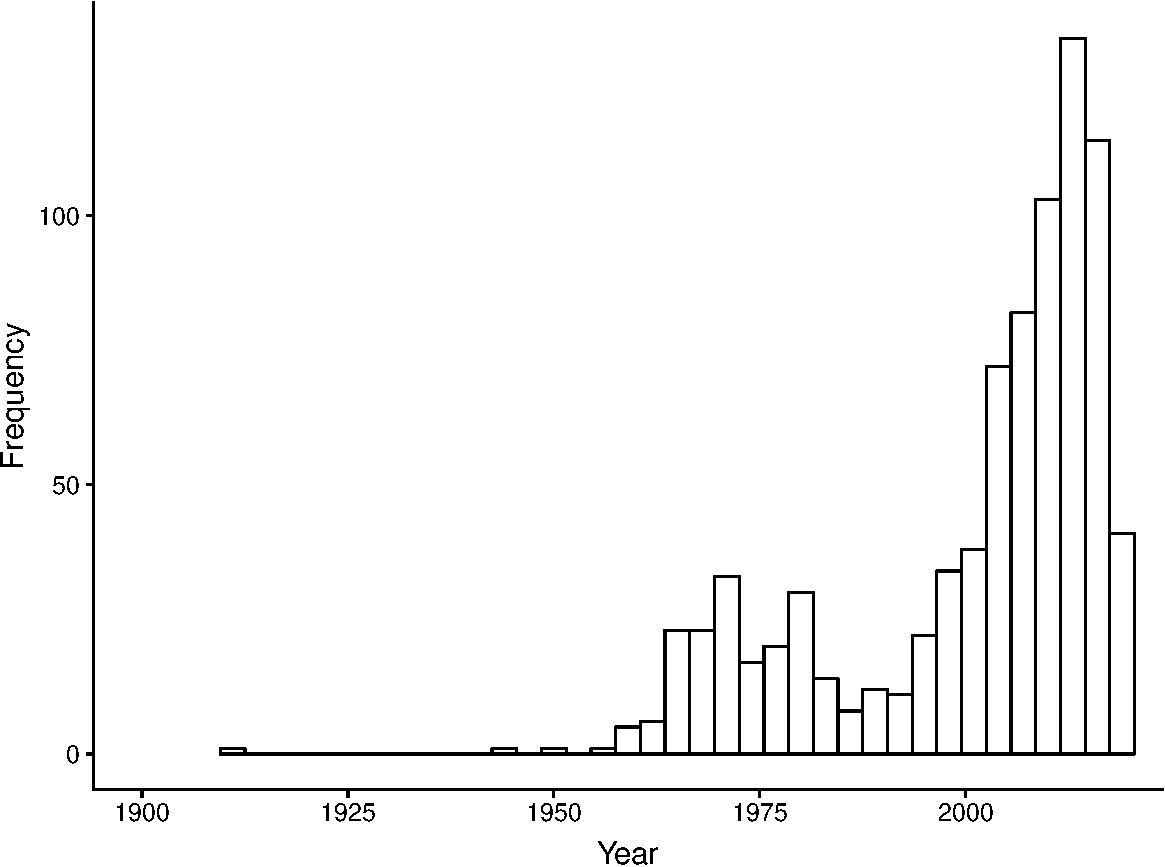
\includegraphics{LAB_files/figure-latex/pub-fig-1.pdf}
\caption{\label{fig:pub-fig}Overall publication frequency across years.}
\end{figure}

\subsubsection{Stimuli}\label{stimuli}

Stimuli are presented in Table \ref{tab:lang-table}, and a review of
this table indicated that the publication of word stimuli was slightly
under half the dataset (48.0), which has quite a large range of quantity
of stimuli from only ten words to a large corpus of over 500 million
words. The wide range of data includes these corpora materials, but
there are very large word norming projects outside of the corpora
included in the LAB. Other types of word stimuli also appear commonly in
the LAB data such as categories, letters, and word pairs. Because
linguistic data was of particular interest, we selected publications
based on words and word pairs, and plotted the number of stimuli
presented in the paper to examine big data trends. These data were
broken down by set size in Figure \ref{fig:word-fig}. The upper left
hand quadrant shows all stimuli across years, and the big data
publications stand out in the last fifteen years of publications. This
data was then further broken down into small datasets (\textless{}1,000
stimuli; upper right quadrant), medium datasets (1,000 - 1,000,000
stimuli; bottom left quadrant), and large datasets (1,000,000+ although
there is a large jump between medium and large as most data is either
half million or less or a million or more; bottom right quadrant). The
small dataset graph shows that these publications are common across
time, while the bottom two quadrants are more telling for the
megastudies trend investigation. As with languages and tags (below), we
see an increase in the number of medium and very large datasets across
the years where the lone large dataset outlier in the early years is the
Brown Corpus (Kucera \& Francis, 1967).

\begin{verbatim}
## Warning: Removed 103 rows containing missing values (geom_point).
\end{verbatim}

\begin{figure}
\centering
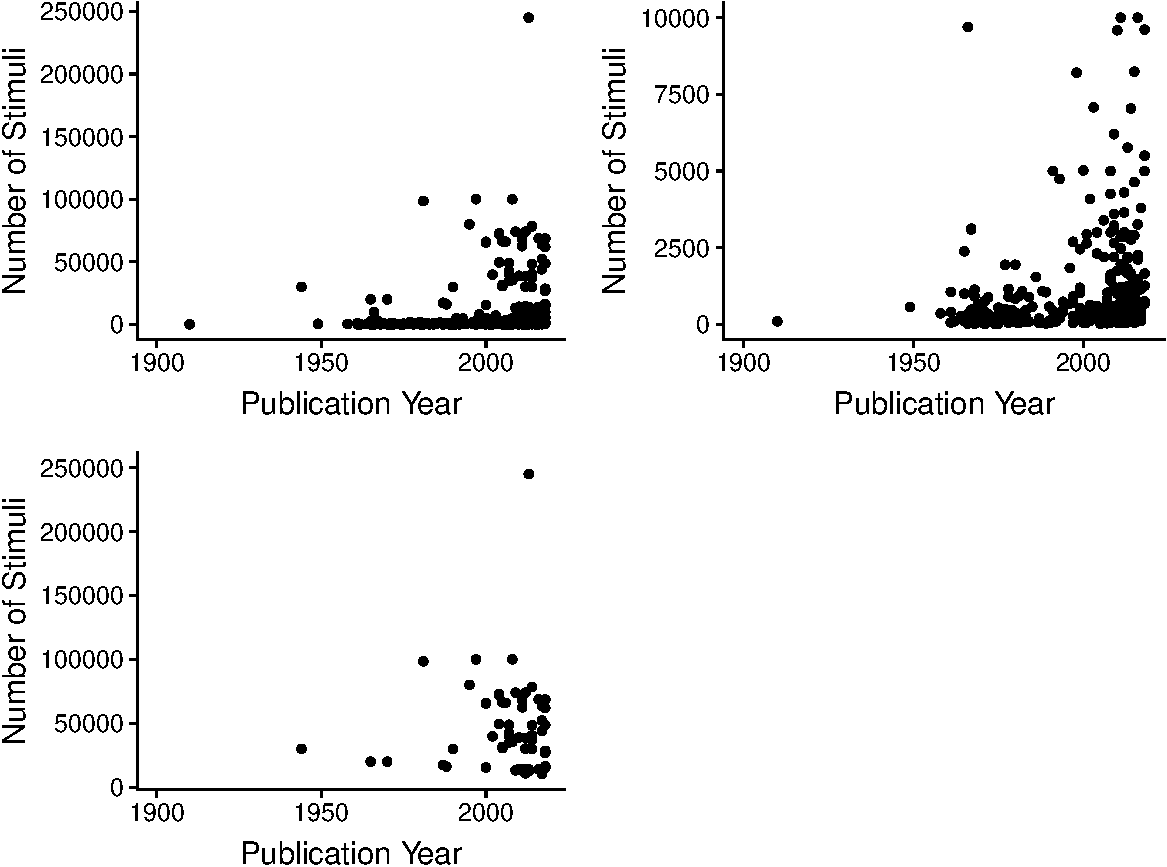
\includegraphics{LAB_files/figure-latex/word-fig-1.pdf}
\caption{\label{fig:word-fig}Number of word stimuli plotted across years.
Top left quandrant includes all word stimuli. Top right quadrant
includes word stimuli ranging up to 1000 words, bottom left quadrant
portrays stimuli counts from 1000 to one million, and bottom right
quadrant indicates all stimuli above one million.}
\end{figure}

\subsubsection{Languages}\label{languages}

The variety and number of languages for stimuli provided an encouraging
picture of the growth and diversity of psycholinguistic stimuli, as seen
in Table \ref{tab:lang-table}. Many articles include multiple languages
( 5.2), as well as the inclusion of both Portuguese ( 2.1) and Spanish (
7.6), French ( 5.7), and German ( 4.2). To examine trends, the English
only articles were filtered out of the dataset since they were the
majority of publications (56.7) and were published across all years
present in this data. Of the 283 non-English publications, 37 included
multiple langauges, and 21 of these were published after 2010.
Additionally, the last ten years (2008 and later) have seen an explosion
of publications in non-English languages, 186, with 21 in 2017 alone.

\subsubsection{Tags}\label{tags}

\begin{figure}
\centering
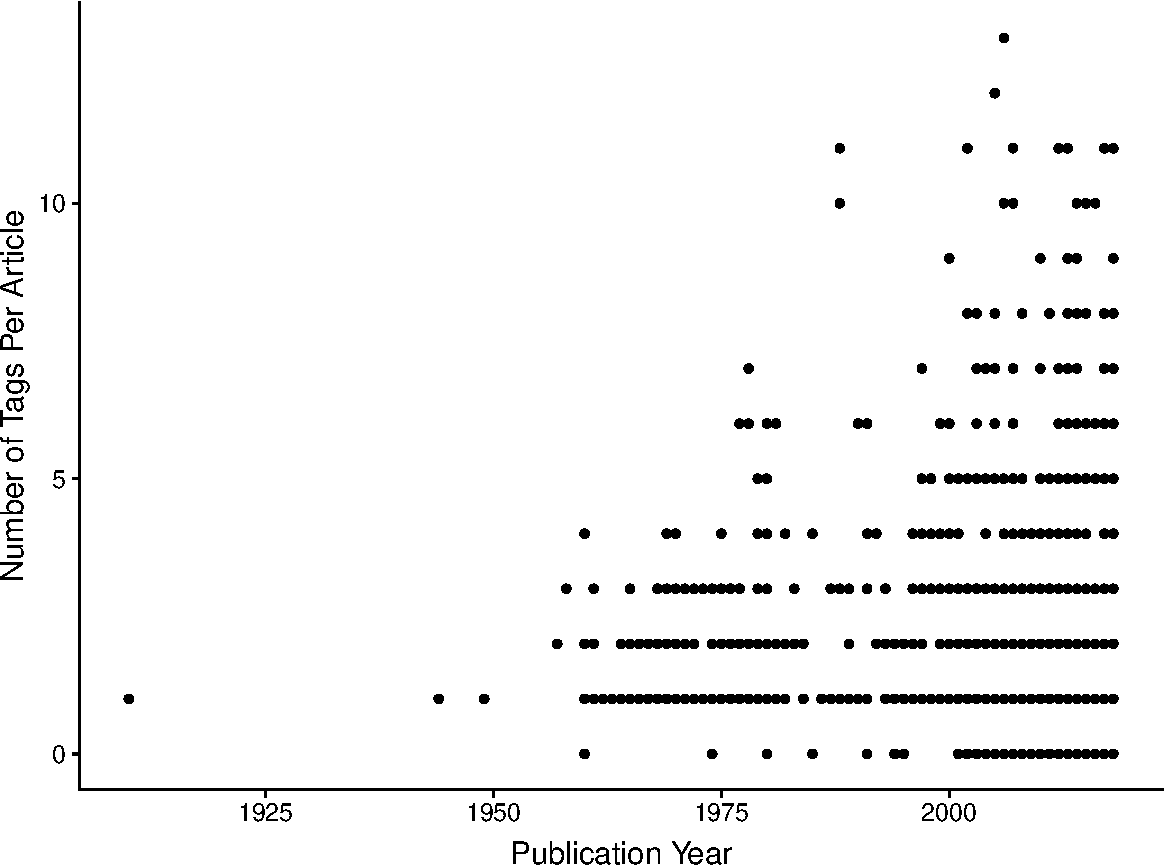
\includegraphics{LAB_files/figure-latex/tag-fig-1.pdf}
\caption{\label{fig:tag-fig}Tag publication frequency across years.}
\end{figure}

Table \ref{tab:tag-table} displays the number, percentages, correlations
of tags across year, and descriptions of tags. Undoubtedly, these tags
represent changes in terminology over time, and some could be combined
or recoined. However, even if low frequency (\emph{N} \textless{} 10;
nine tags) tags were excluded, thirty-seven different tags were used to
describe the types of psycholinguistic data. Many of these tags can be
considered individual research areas, and the sizeable number of
different options indicates how complex and diverse the field has become
since the publication of free association norms in 1910 (Kent \&
Rosanoff, 1910).

The total number of tags for each publication was then tallied, and this
data was plotted in Figure \ref{tab:tag-fig} to visualize if the number
of variables included in a study has grown over time (\emph{M} = 2.69,
\emph{SD} = 2.27). The correlation between total tags and year was
\texttt{rapa\_print(cor.test(master\$totaltag,\ master\$year,\ use\ =\ "pairwise.complete.obs"))\$full\_result},
indicating a small increase in total tags used over time. Even
considering the larger number of publications in the 2000s versus 1950s
to 1970s, it appeared that the number of keywords for articles was also
slowly growing over time. This trend may indicate the evolution in
computing possibilities to be able to publish large amounts of data, but
also may indicate a desire to combine datasets so that even more stimuli
may be considered at once for modeling or experiment creation.

Next, tags with at least a sample of 30 publications were investigated
individually for trends across time (correlations presented in Table
\ref{tab:tag-table}). Individual histograms can be created by clicking
on the Tags Per Year link online, which show the total frequency of the
selected tag by year. Some small positive trends were found, such as the
increase in arousal, age of acquisition, syllables, familiarity, and
valence norms. Intriguingly, meaningfulness and association both showed
negative correlations, but these correlations can be understood as an
artifact of the publication of a book on association norms in the 1970s
(Postman \& Keppel, 1970), as well as a recent drop off of in the small
but steady use of meaningfulness. These small correlations may partially
be explained by the sheer number and variation of data available in the
LAB portal, as one would expect the number of frequency tags to increase
with the recent SUBTLEX publications. Indeed, if the frequency tags were
plotted by year an increase across the last decade (16 in 2010 and 2013,
and 21 in 2014) can be found. Readers are encouraged to view the
individual graphs for tags to investigate the change of keyword
publication over time, including the rise and demise of several research
areas. For example, confusion matrices heyday appeared to range from the
early 70s to the mid 80s, while arousal norms do not make a consistent
appearance until the late 90s.

\section{Conclusion}\label{conclusion}

This article had two main purposes: 1) to present the LAB dataset and
portal as an annotated bibliography and searchable tool for researchers,
and 2) to view trends in psycholinguistic research with an eye toward
big data. We believe the LAB website will be a useful channel for all
levels of researchers, from graduate students looking for experimental
stimuli to design their experiments, to the familiar investigator who
wishes to dig deeper into the diverse choices offered. Further, while
the majority of publications occur in one particular journal, the LAB
allows someone to find articles they may have missed in other areas with
the advantage of being collected into one location. User-friendly search
tools are provided to aide in searching for specific languages, stimuli,
or keywords, as well as multiple outputs for easy copying into Excel or
SPSS. While this article's statistics will become dated with the updates
to the LAB, dynamic tables and graphs are provided online to see the
current status of the field. Lastly, we encourage users to actively
report errors and suggest updates for the LAB dataset as a way to crowd
source information that is surely missing, especially in non-English
languages.

In the introduction, we provided two examples of current megastudies
(SUBTLEX and the Lexicon projects), in addition to how researchers might
collect big data through Mechanical Turk or Twitter. This article
stepped back from looking at individual, large studies or ways to
collect data to use the information provided by publications as a window
into the fluctuations of the field. Megastudies have become a prevalent
topic, but data could have revealed that this popularity was due to
recent publication of a small subset of articles. Instead, analyses
showed that not only are the numbers of publications accumulating, but
the sizes of datasets are also growing in tandem. Megastudies
specifically focus on large datasets, but big data can also be indicated
here by the divergence in languages available, number of places to
publish such data, and the increasing number of keywords for articles
across years. Time will tell if these trends can and will continue or if
certain areas will see a confusion matrix type decline after many large
datasets are published. With the move of traditional lab experiments to
smartphone and tablet technology (Dufau et al., 2011), it seems likely
that researchers in psycholinguistics will continue to find new and
creative ways to modernize the field.

\newpage

\section{References}\label{references}

\setlength{\parindent}{-0.5in} \setlength{\leftskip}{0.5in}

\hypertarget{refs}{}
\hypertarget{ref-Adelman2006}{}
Adelman, J. S., Brown, G. D. A., \& Quesada, J. F. (2006). Contextual
Diversity Not Word Frequency Determines Time To Read. \emph{Psychology},
\emph{17}(Cd), 814--823. Retrieved from
\url{http://pss.sagepub.com/content/17/9/814.short}

\hypertarget{ref-R-papaja}{}
Aust, F., \& Barth, M. (2017). \emph{papaja: Create APA manuscripts with
R Markdown}. Retrieved from \url{https://github.com/crsh/papaja}

\hypertarget{ref-Baayen}{}
Baayen, R. H., Piepenbrock, R., Gulikers, L., \& Linguistic Data
Consortium. (n.d.). The CELEX Lexical Database (CD-ROM). Philadelphia,
PA:

\hypertarget{ref-Balota2004}{}
Balota, D. A., Cortese, M. J., Sergent-Marshall, S. D., Spieler, D. H.,
\& Yap, M. J. (2004). Visual word recognition of single-syllable words.
\emph{Journal of Experimental Psychology: General}, \emph{133}(2),
283--316.
doi:\href{https://doi.org/10.1037/0096-3445.133.2.283}{10.1037/0096-3445.133.2.283}

\hypertarget{ref-Balota2007}{}
Balota, D. A., Yap, M. J., Cortese, M. J., Hutchison, K. A., Kessler,
B., Loftis, B., \ldots{} Treiman, R. (2007). The english lexicon
project. \emph{Behavior Research Methods}, \emph{39}(3), 445--459.
doi:\href{https://doi.org/10.3758/BF03193014}{10.3758/BF03193014}

\hypertarget{ref-Barca2002}{}
Barca, L., Burani, C., \& Arduino, L. S. (2002). Word naming times and
psycholinguistic norms for Italian nouns. \emph{Behavior Research
Methods, Instruments, \& Computers : A Journal of the Psychonomic
Society, Inc}, \emph{34}(3), 424--434.
doi:\href{https://doi.org/10.3758/BF03195471}{10.3758/BF03195471}

\hypertarget{ref-Boudelaa2010}{}
Boudelaa, S., \& Marslen-Wilson, W. D. (2010). Aralex: A lexical
database for modern standard Arabic. \emph{Behavior Research Methods},
\emph{42}(2), 481--487.
doi:\href{https://doi.org/10.3758/BRM.42.2.481}{10.3758/BRM.42.2.481}

\hypertarget{ref-Bradshaw1984}{}
Bradshaw, J. L. (1984). A guide to norms, ratings, and lists.
\emph{Memory \& Cognition}, \emph{12}(2), 202--206.
doi:\href{https://doi.org/10.3758/BF03198435}{10.3758/BF03198435}

\hypertarget{ref-Brodeur2010}{}
Brodeur, M. B., Dionne-Dostie, E., Montreuil, T., \& Lepage, M. (2010).
The bank of standardized stimuli (BOSS), a new set of 480 normative
photos of objects to be used as visual stimuli in cognitive research.
\emph{PLoS ONE}, \emph{5}(5).
doi:\href{https://doi.org/10.1371/journal.pone.0010773}{10.1371/journal.pone.0010773}

\hypertarget{ref-Brysbaert2009}{}
Brysbaert, M., \& New, B. (2009). Moving beyond Kučera and Francis: A
critical evaluation of current word frequency norms and the introduction
of a new and improved word frequency measure for American English.
\emph{Behavior Research Methods}, \emph{41}(4), 977--990.
doi:\href{https://doi.org/10.3758/BRM.41.4.977}{10.3758/BRM.41.4.977}

\hypertarget{ref-Brysbaert2011}{}
Brysbaert, M., Buchmeier, M., Conrad, M., Jacobs, A. M., Bölte, J., \&
Böhl, A. (2011). The word frequency effect: A review of recent
developments and implications for the choice of frequency estimates in
German. \emph{Experimental Psychology}, \emph{58}(5), 412--424.
doi:\href{https://doi.org/10.1027/1618-3169/a000123}{10.1027/1618-3169/a000123}

\hypertarget{ref-Brysbaert2013}{}
Brysbaert, M., Warriner, A. B., \& Kuperman, V. (2014). Concreteness
ratings for 40 thousand generally known English word lemmas.
\emph{Behavior Research Methods}, \emph{46}(3), 904--911.
doi:\href{https://doi.org/10.3758/s13428-013-0403-5}{10.3758/s13428-013-0403-5}

\hypertarget{ref-Buchanan2018}{}
Buchanan, E. M., \& Scofield, J. E. (2018). Methods to detect low
quality data and its implication for psychological research.
\emph{Behavior Research Methods}.
doi:\href{https://doi.org/10.3758/s13428-018-1035-6}{10.3758/s13428-018-1035-6}

\hypertarget{ref-Buchanan2013}{}
Buchanan, E. M., Holmes, J. L., Teasley, M. L., \& Hutchison, K. A.
(2013). English semantic word-pair norms and a searchable Web portal for
experimental stimulus creation. \emph{Behavior Research Methods},
\emph{45}(3), 746--757.
doi:\href{https://doi.org/10.3758/s13428-012-0284-z}{10.3758/s13428-012-0284-z}

\hypertarget{ref-Buhrmester2011}{}
Buhrmester, M., Kwang, T., Gosling, S. D., Buhrmester, M., Kwang, T., \&
Gosling, S. D. (2011). Amazon's Mechanical Turk: A New Source of
Inexpensive, Yet High-Quality, Data?, \emph{6}(1), 3--5.

\hypertarget{ref-Burgess1998}{}
Burgess, C., \& Livesay, K. (1998). The effect of corpus size in
predicting reaction time in a basic word recognition task: Moving on
from Kučera and Francis. \emph{Behavior Research Methods, Instruments,
and Computers}, \emph{30}(2), 272--277.
doi:\href{https://doi.org/10.3758/BF03200655}{10.3758/BF03200655}

\hypertarget{ref-Cai2010}{}
Cai, Q., \& Brysbaert, M. (2010). SUBTLEX-CH: Chinese word and character
frequencies based on film subtitles. \emph{PLoS ONE}, \emph{5}(6).
doi:\href{https://doi.org/10.1371/journal.pone.0010729}{10.1371/journal.pone.0010729}

\hypertarget{ref-R-shiny}{}
Chang, W., Cheng, J., Allaire, J., Xie, Y., \& McPherson, J. (2017).
\emph{Shiny: Web application framework for r}. Retrieved from
\url{https://CRAN.R-project.org/package=shiny}

\hypertarget{ref-Cohen-Shikora2013}{}
Cohen-Shikora, E. R., Balota, D. A., Kapuria, A., \& Yap, M. J. (2013).
The past tense inflection project (PTIP): Speeded past tense
inflections, imageability ratings, and past tense consistency measures
for 2,200 verbs. \emph{Behavior Research Methods}, \emph{45}(1),
151--159.
doi:\href{https://doi.org/10.3758/s13428-012-0240-y}{10.3758/s13428-012-0240-y}

\hypertarget{ref-Cree2003}{}
Cree, G. S., \& McRae, K. (2003). Analyzing the Factors Underlying the
Structure and Computation of the Meaning of Chipmunk, Cherry, Chisel,
Cheese, and Cello (and many Other Such Concrete Nouns). \emph{Journal of
Experimental Psychology: General}, \emph{132}(2), 163--201.
doi:\href{https://doi.org/10.1037/0096-3445.132.2.163}{10.1037/0096-3445.132.2.163}

\hypertarget{ref-Cree1999}{}
Cree, G. S., McRae, K., \& McNorgan, C. (1999). An attractor model of
lexical conceptual processing: Simulating semantic priming.
\emph{Cognitive Science}, \emph{23}, 371--414.
doi:\href{https://doi.org/10.1016/S0364-0213(99)00005-1}{10.1016/S0364-0213(99)00005-1}

\hypertarget{ref-Cuetos2011}{}
Cuetos, F., Glez-Nosti, M., Barbon, A., \& Brysbaert, M. (2011).
SUBTLEX-ESP: Spanish word frequencies based on film subtitles.
\emph{Psicologica}, \emph{32}, 133--143.

\hypertarget{ref-DeDeyne2013}{}
De Deyne, S., Navarro, D. J., \& Storms, G. (2013). Better explanations
of lexical and semantic cognition using networks derived from continued
rather than single-word associations. \emph{Behavior Research Methods},
\emph{45}(2), 480--498.
doi:\href{https://doi.org/10.3758/s13428-012-0260-7}{10.3758/s13428-012-0260-7}

\hypertarget{ref-Dimitropoulou2010}{}
Dimitropoulou, M., Duñabeitia, J. A., Avilés, A., Corral, J., \&
Carreiras, M. (2010). Subtitle-based word frequencies as the best
estimate of reading behavior: The case of Greek. \emph{Frontiers in
Psychology}, \emph{1}(DEC), 1--12.
doi:\href{https://doi.org/10.3389/fpsyg.2010.00218}{10.3389/fpsyg.2010.00218}

\hypertarget{ref-Dodds2011}{}
Dodds, P. S., Harris, K. D., Kloumann, I. M., Bliss, C. A., \& Danforth,
C. M. (2011). Temporal patterns of happiness and information in a global
social network: Hedonometrics and Twitter. \emph{PLoS ONE},
\emph{6}(12).
doi:\href{https://doi.org/10.1371/journal.pone.0026752}{10.1371/journal.pone.0026752}

\hypertarget{ref-Dufau2011}{}
Dufau, S., Duñabeitia, J. A., Moret-Tatay, C., McGonigal, A., Peeters,
D., Alario, F. X., \ldots{} Grainger, J. (2011). Smart phone, smart
science: How the use of smartphones can revolutionize research in
cognitive science. \emph{PLoS ONE}, \emph{6}(9), 9--11.
doi:\href{https://doi.org/10.1371/journal.pone.0024974}{10.1371/journal.pone.0024974}

\hypertarget{ref-Guasch2013}{}
Guasch, M., Boada, R., Ferré, P., \& Sánchez-Casas, R. (2013). NIM: A
Web-based Swiss army knife to select stimuli for psycholinguistic
studies. \emph{Behavior Research Methods}, \emph{45}(3), 765--771.
doi:\href{https://doi.org/10.3758/s13428-012-0296-8}{10.3758/s13428-012-0296-8}

\hypertarget{ref-VanHeuven2014}{}
Heuven, W. J. van, Mandera, P., Keuleers, E., \& Brysbaert, M. (2014).
SUBTLEX-UK: A new and improved word frequency database for British
English. \emph{Quarterly Journal of Experimental Psychology},
\emph{67}(6), 1176--1190.
doi:\href{https://doi.org/10.1080/17470218.2013.850521}{10.1080/17470218.2013.850521}

\hypertarget{ref-Hutchison2013}{}
Hutchison, K. A., Balota, D. A., Neely, J. H., Cortese, M. J.,
Cohen-Shikora, E. R., Tse, C.-S., \ldots{} Buchanan, E. M. (2013). The
semantic priming project. \emph{Behavior Research Methods},
\emph{45}(4), 1099--1114.
doi:\href{https://doi.org/10.3758/s13428-012-0304-z}{10.3758/s13428-012-0304-z}

\hypertarget{ref-Jasmin2012}{}
Jasmin, K., \& Casasanto, D. (2012). The QWERTY Effect: How typing
shapes the meanings of words. \emph{Psychonomic Bulletin \& Review},
\emph{19}(3), 499--504.
doi:\href{https://doi.org/10.3758/s13423-012-0229-7}{10.3758/s13423-012-0229-7}

\hypertarget{ref-Kent1910}{}
Kent, G. H., \& Rosanoff, A. J. (1910). A study of association in
insanity. \emph{The American Journal of Psychiatry}, \emph{67},
317--390.
doi:\href{https://doi.org/10.1037/13767-000}{10.1037/13767-000}

\hypertarget{ref-Keuleers2010}{}
Keuleers, E., Brysbaert, M., \& New, B. (2010). SUBTLEX-NL: A new
measure for Dutch word frequency based on film subtitles. \emph{Behavior
Research Methods}, \emph{42}(3), 643--650.
doi:\href{https://doi.org/10.3758/BRM.42.3.643}{10.3758/BRM.42.3.643}

\hypertarget{ref-Keuleers2012}{}
Keuleers, E., Lacey, P., Rastle, K., \& Brysbaert, M. (2012). The
British Lexicon Project: Lexical decision data for 28,730 monosyllabic
and disyllabic English words. \emph{Behavior Research Methods},
\emph{44}(1), 287--304.
doi:\href{https://doi.org/10.3758/s13428-011-0118-4}{10.3758/s13428-011-0118-4}

\hypertarget{ref-Kloumann2012}{}
Kloumann, I. M., Danforth, C. M., Harris, K. D., Bliss, C. A., \& Dodds,
P. S. (2012). Positivity of the English language. \emph{PLoS ONE},
\emph{7}(1), 0--6.
doi:\href{https://doi.org/10.1371/journal.pone.0029484}{10.1371/journal.pone.0029484}

\hypertarget{ref-Kucera1967}{}
Kucera, H., \& Francis, W. N. (1967). \emph{Computational analysis of
present-day American English.} Providence, RI: Brown University Press.

\hypertarget{ref-Kuperman2012}{}
Kuperman, V., Stadthagen-Gonzalez, H., \& Brysbaert, M. (2012).
Age-of-acquisition ratings for 30,000 English words. \emph{Behavior
Research Methods}, \emph{44}(4), 978--990.
doi:\href{https://doi.org/10.3758/s13428-012-0210-4}{10.3758/s13428-012-0210-4}

\hypertarget{ref-Landauer1997}{}
Landauer, T. K., \& Dumais, S. T. (1997). A solution to Plato's problem:
The latent semantic analysis theory of acquisition, induction, and
representation of knowledge. \emph{Psychological Review}, \emph{104}(2),
211--240.
doi:\href{https://doi.org/10.1037//0033-295X.104.2.211}{10.1037//0033-295X.104.2.211}

\hypertarget{ref-Lete2004}{}
Lété, B., \& Sprenger-Charolles, L. (2004). MANULEX: A lexical database
from French readers. \emph{Behaviour Research Methods Instruments and
Computers}, \emph{36}(1), 156--166.

\hypertarget{ref-Maki2004}{}
Maki, W. S., McKinley, L. N., \& Thompson, A. G. (2004). Semantic
distance norms computed from an electronic dictionary (WordNet).
\emph{Behavior Research Methods, Instruments, \& Computers},
\emph{36}(3), 421--431.
doi:\href{https://doi.org/10.3758/BF03195590}{10.3758/BF03195590}

\hypertarget{ref-Mason2012}{}
Mason, W., \& Suri, S. (2012). Conducting behavioral research on
Amazon's Mechanical Turk. \emph{Behavior Research Methods},
\emph{44}(1), 1--23.
doi:\href{https://doi.org/10.3758/s13428-011-0124-6}{10.3758/s13428-011-0124-6}

\hypertarget{ref-McRae1997}{}
McRae, K., De Sa, V. R., \& Seidenberg, M. S. (1997). On the Nature and
Scope of Featural Representations of Word Meaning. \emph{Journal of
Experimental Psychology: General}, \emph{126}(2), 99--130.
doi:\href{https://doi.org/10.1037/0096-3445.126.2.99}{10.1037/0096-3445.126.2.99}

\hypertarget{ref-Miller2003}{}
Miller, G. A. (2003). The cognitive revolution: A historical
perspective. \emph{Trends in Cognitive Sciences}, \emph{7}, 141--144.
doi:\href{https://doi.org/10.1016/S1364-6613(03)00029-9}{10.1016/S1364-6613(03)00029-9}

\hypertarget{ref-Moss2002}{}
Moss, H. E., Tyler, L. K., \& Devlin, J. T. (2002). The emergence of
category-specific deficits in a distribuited semantic system.

\hypertarget{ref-Nelson2004}{}
Nelson, D. L., McEvoy, C. L., \& Schreiber, T. A. (2004). The University
of South Florida free association, rhyme, and word fragment norms.
\emph{Behavior Research Methods, Instruments, \& Computers},
\emph{36}(3), 402--407.
doi:\href{https://doi.org/10.3758/BF03195588}{10.3758/BF03195588}

\hypertarget{ref-New2007}{}
New, B., Brysbaert, M., Veronis, J., \& Pallier, C. (2007). The use of
film subtitles to estimate word frequencies. \emph{Applied
Psycholinguistics}, \emph{28}(4), 661--677.
doi:\href{https://doi.org/10.1017/S014271640707035X}{10.1017/S014271640707035X}

\hypertarget{ref-Pexman2003}{}
Pexman, P. M., Holyk, G. G., \& Monfils, M.-H. (2003).
Number-of-features effects and semantic processing. \emph{Memory \&
Cognition}, \emph{31}(6), 842--855.
doi:\href{https://doi.org/10.3758/BF03196439}{10.3758/BF03196439}

\hypertarget{ref-Postman1970}{}
Postman, L., \& Keppel, G. (1970). \emph{Norms of word association.} New
York: Academic Press.

\hypertarget{ref-Proctor1999}{}
Proctor, R. W., \& Kim-Phuong, L. V. (1999). Index of norms and ratings
published in the Psychonomic Society journals. \emph{Behavior Research
Methods, Instruments, and Computers}, \emph{31}(4), 659--667.
doi:\href{https://doi.org/10.3758/BF03200742}{10.3758/BF03200742}

\hypertarget{ref-Rayner1986}{}
Rayner, K., \& Duffy, S. A. (1986). Lexical complexity and fixation
times in reading: Effects of word frequency, verb complexity, and
lexical ambiguity. \emph{Memory \& Cognition}, \emph{14}(3), 191--201.
doi:\href{https://doi.org/10.3758/BF03197692}{10.3758/BF03197692}

\hypertarget{ref-Rogers2004}{}
Rogers, T. T., \& McClelland, J. L. (2004). \emph{Semantic cognition: A
parallel distributed processing approach}. MIT Press.

\hypertarget{ref-Snodgrass1980}{}
Snodgrass, J. G., \& Vanderwart, M. (1980). A standardized set of 260
pictures: Norms for name agreement, image agreement, familiarity, and
visual complexity. \emph{Journal of Experimental Psychology: Human
Learning and Memory}, \emph{6}(2), 174--215.
doi:\href{https://doi.org/10.1037/0278-7393.6.2.174}{10.1037/0278-7393.6.2.174}

\hypertarget{ref-Soares2014}{}
Soares, A. P., Medeiros, J. C., Simões, A., Machado, J., Costa, A.,
Iriarte, Á., \ldots{} Comesaña, M. (2014). ESCOLEX: A grade-level
lexical database from European Portuguese elementary to middle school
textbooks. \emph{Behavior Research Methods}, \emph{46}(1), 240--253.
doi:\href{https://doi.org/10.3758/s13428-013-0350-1}{10.3758/s13428-013-0350-1}

\hypertarget{ref-Sze2014}{}
Sze, W. P., Rickard Liow, S. J., \& Yap, M. J. (2014). The Chinese
Lexicon Project: A repository of lexical decision behavioral responses
for 2,500 Chinese characters. \emph{Behavior Research Methods},
\emph{46}(1), 263--273.
doi:\href{https://doi.org/10.3758/s13428-013-0355-9}{10.3758/s13428-013-0355-9}

\hypertarget{ref-Vaughan2004}{}
Vaughan, J. (2004). Editorial: a web-based archive of norms, stimuli,
and data. \emph{Behavior Research Methods, Instruments, \& Computers : A
Journal of the Psychonomic Society, Inc}, \emph{36}(3), 363--370.
doi:\href{https://doi.org/10.3758/BF03195583}{10.3758/BF03195583}

\hypertarget{ref-Vigliocco2004}{}
Vigliocco, G., Vinson, D. P., Lewis, W., \& Garrett, M. F. (2004).
Representing the meanings of object and action words: The featural and
unitary semantic space hypothesis. \emph{Cognitive Psychology},
\emph{48}(4), 422--488.
doi:\href{https://doi.org/10.1016/j.cogpsych.2003.09.001}{10.1016/j.cogpsych.2003.09.001}

\hypertarget{ref-Vinson2003}{}
Vinson, D. P., Vigliocco, G., Cappa, S., \& Siri, S. (2003). The
breakdown of semantic knowledge: Insights from a statistical model of
meaning representation. \emph{Brain and Language}, \emph{86}(3),
347--365.
doi:\href{https://doi.org/10.1016/S0093-934X(03)00144-5}{10.1016/S0093-934X(03)00144-5}

\hypertarget{ref-Vo2009}{}
Vo, M. L. H., Conrad, M., Kuchinke, L., Urton, K., Hofmann, M. J., \&
Jacobs, A. M. (2009). The Berlin Affective Word List Reloaded (BAWL-R).
\emph{Behavior Research Methods}, \emph{41}(2), 534--538.
doi:\href{https://doi.org/10.3758/BRM.41.2.534}{10.3758/BRM.41.2.534}

\hypertarget{ref-Warriner2013}{}
Warriner, A. B., Kuperman, V., \& Brysbaert, M. (2013). Norms of
valence, arousal, and dominance for 13,915 English lemmas.
\emph{Behavior Research Methods}, \emph{45}(4), 1191--1207.
doi:\href{https://doi.org/10.3758/s13428-012-0314-x}{10.3758/s13428-012-0314-x}

\hypertarget{ref-Yap2010}{}
Yap, M. J., Rickard Liow, S. J., Jalil, S. B., \& Faizal, S. S. B.
(2010). The malay lexicon project: A database of lexical statistics for
9,592 words. \emph{Behavior Research Methods}, \emph{42}(4), 992--1003.
doi:\href{https://doi.org/10.3758/BRM.42.4.992}{10.3758/BRM.42.4.992}

\hypertarget{ref-Yap2011}{}
Yap, M. J., Tan, S. E., Pexman, P. M., \& Hargreaves, I. S. (2011). Is
more always better? Effects of semantic richness on lexical decision,
speeded pronunciation, and semantic classification. \emph{Psychonomic
Bulletin and Review}, \emph{18}(4), 742--750.
doi:\href{https://doi.org/10.3758/s13423-011-0092-y}{10.3758/s13423-011-0092-y}

\hypertarget{ref-Zevin2002}{}
Zevin, J., \& Seidenberg, M. (2002). Age of acquisition effects in word
reading and other tasks. \emph{Journal of Memory and Language},
\emph{47}(1), 1--29.
doi:\href{https://doi.org/10.1006/jmla.2001.2834}{10.1006/jmla.2001.2834}






\end{document}
